%!TEX root = ../report.tex


\chapter{Visual Design}\label{ch:visual-design}

To create a visually aesthetic application we have taken into account several preparation steps upfront. In this chapter
we will go into more detail on which steps have been accomplished and how they helped us to implement our frontend parts
later on.


\section{Laws of UX}\label{sec:laws-of-ux}

\enquote{Laws of UX is a collection of the maxims and principles that designers can consider when building user interfaces.
It was created by Jon Yablonski.}~\cite{lawsofux}.

\subsection{Aesthetic Usability Effect}\label{subsec:aestetic-usability-effect}

Research has shown that aesthetically pleasing design is often perceived as more user-friendly and usable.
People tend to be more error tolerant in case of small bugs.
Further, people tent to link positive feelings with aesthetically pleasing things.
Therefore, if an aesthetically pleasing user interface is present, the user will automatically tend to link a positive
feeling to the application.
Down the road this will most-likely lead to more time the user spent with the application which should be the ultimate
goal of application creators~\cite{lawsofuxAUE}.

\subsection{Doherty Threshold}\label{subsec:doherty-threshold}
According to a research done by Walter J. Doherty and Ahrvind J. Thadani in 1982, the average response time of a
computer should not exceed 400 milliseconds.
The research has shown that if a user interacts with a system responding in 400 milliseconds or less will be perceived
as a fast and reliable system.
This outcome has an addictive effect on the user leading to increased time spend within the application.
Lastly, the more time the users spends using the application, the more effective will be the addictive
force~\cite{lawsofuxDT}.

\subsection{Fitt's Law}\label{subsec:fitt's-law}
The psychologist Paul Fitts examined the interaction of humans with targets.
His study showed that there is a correlation between navigation to a target and its size.
Moving fast to a small target is more error prone than moving fast to a large target due to the speed-accuracy trade-off.
This design principle is widely accepted in user experience design and commonly applied when designing user interfaces.
For instance, interactive buttons to trigger an event are often large to be easily and fast accessible.
This applies specifically to interfaces which are utilized on touch devices to enable the user to easily interact with
their fingers.
Additionally, the distance between objects where the user attention lies, and the task trigger (e.g.\ a button) should be
as small as possible to eliminate the need of fast interaction which leads to a decreased accuracy~\cite{lawsofuxFL}.

\subsection{Hick's Law}\label{subsec:hick's-law}
Hick's law is the outcome of a psychologist team that analyzed the correlation of a range of elements, and an
individual's reaction time.
The team found out that the more choices we have, the longer it takes to choose on of the available choices.
In user experience design this should be taken into account.
For instance, if there are 20 buttons visible to the interacting user, the user would need a significant duration to
come to a final choice which action he wants to perform.
Therefore, the user shall only be given the options which are really required.
Displaying all options possible would only lead to confusion and long reaction times conflicting with the
\textbf{\hyperref[subsec:doherty-threshold]{Doherty Threshold}}~\cite{lawsofuxHL}.

\subsection{Laws of UX Conclusion}\label{subsec:laws-of-ux-conclusion}
The laws of \ac{ux} are the most recognized and utilizable laws of designing a sophisticated and ingenious \ac{ux}
along with an aesthetically pleasing \ac{ui}.
Jon Yablonski created a collection of the most important psychological tricks and behaviours and applied them to
\ac{ux} and \ac{ui}.
We tried to apply the above mentioned laws in any way possible as we designed the \ac{ui} for Trale Messenger.
The next section will go into more detail on how we approached the visual design.

\section{Styleguide}\label{sec:styleguide}
A styleguide is a useful resource for front-end developers to start the implementation of the \ac{ui}.
It is a collection of information, rules, restrictions and hints on how the \ac{ui} should be implemented.
The following sub sections will dive into the actual guidelines we defined for the front-end developers.

\subsection{Grid \& Measurements}\label{subsec:grid-and-measurements}

It started with defining a grid and measurements guide for arranging all application components. For this we created a
grid visualization (Figure~\ref{fig:grid}).

\begin{figure}[!ht]
    \centering
    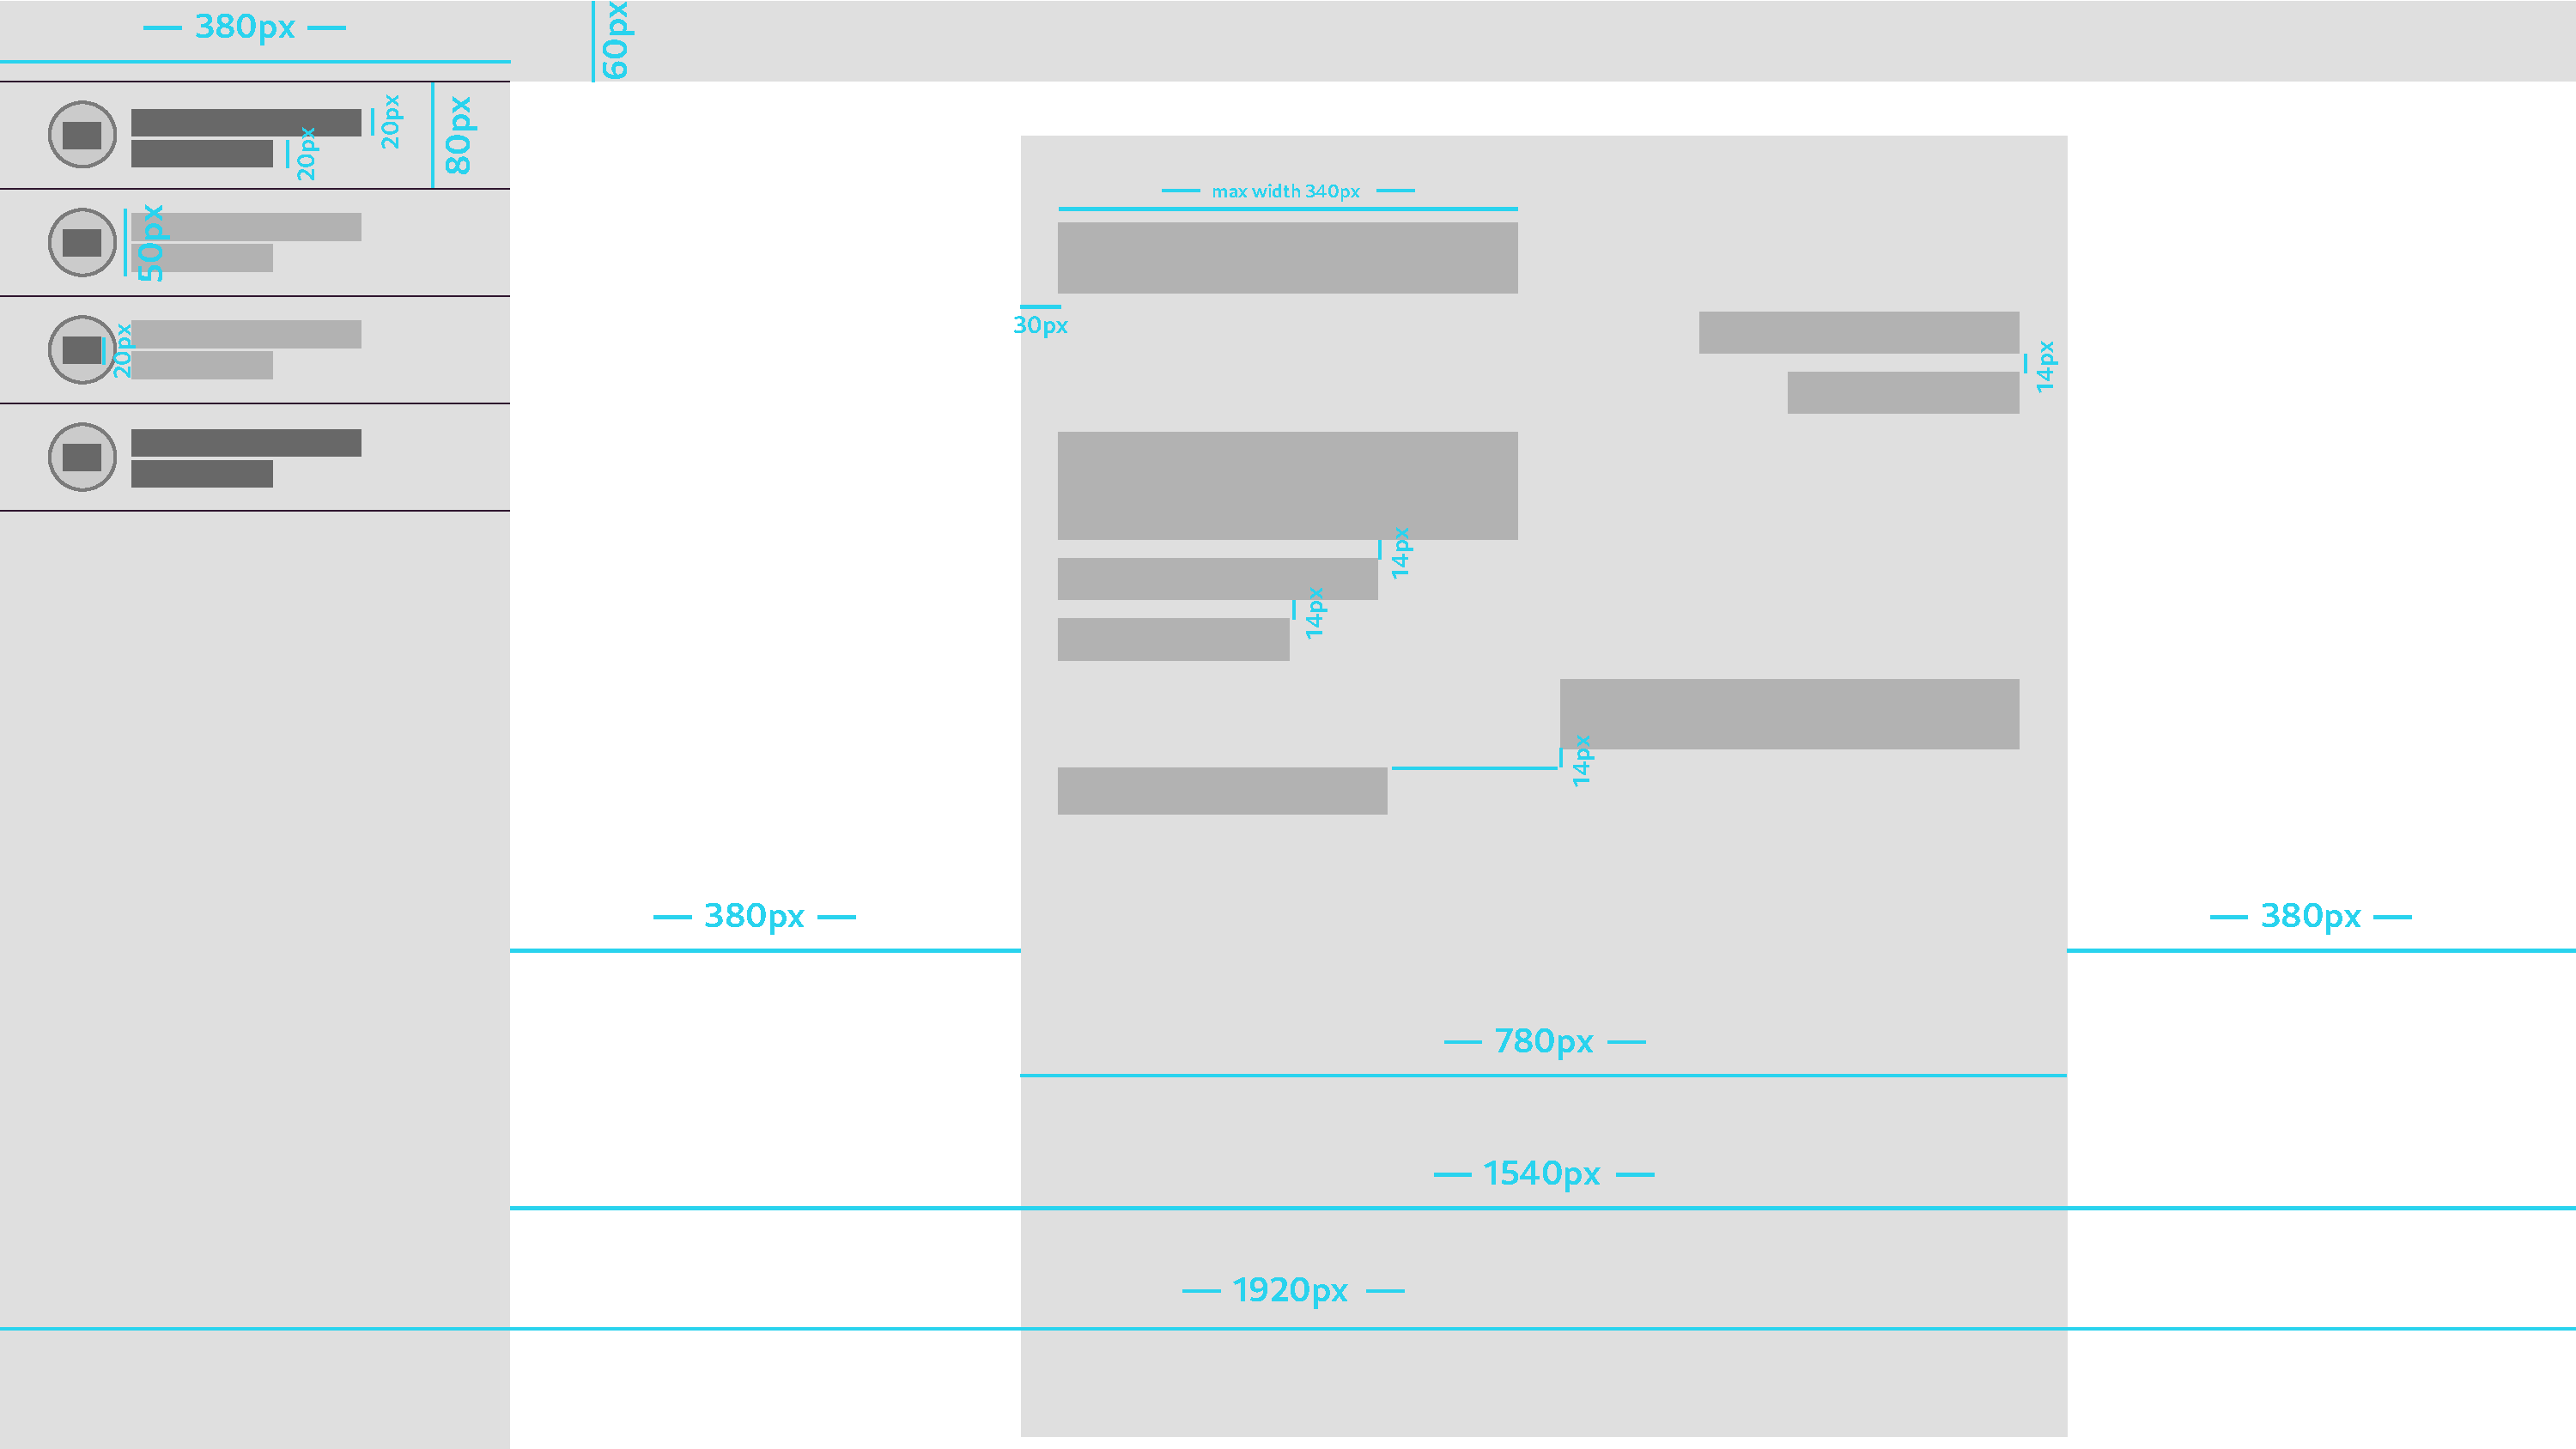
\includegraphics[width=1.0\textwidth]{./graphics/grid}
    \caption{Grid and Measurements visualization}
    \label{fig:grid}
\end{figure}

\subsection{Message Styling}\label{subsec:message-styling}

\begin{figure}[ht]
    \caption{Message Styling Design Reference}
    
\includegraphics[width=1.0\textwidth]{./graphics/messages}\label{fig:figure2}
\end{figure}

\subsection{Messages States}\label{subsec:messages-states}
\begin{figure}[ht]
    \caption{Message States Design Reference}
    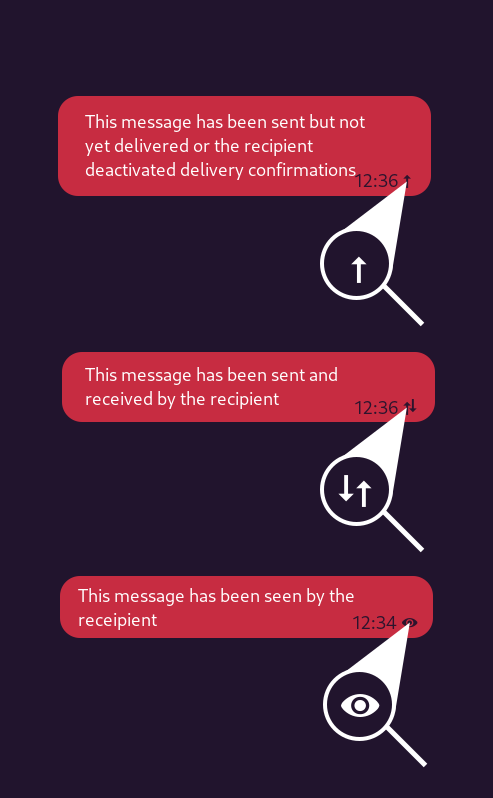
\includegraphics[width=1.0\textwidth]{./graphics/message-states}\label{fig:figure3}
\end{figure}

\subsection{Color Palette}\label{subsec:color-palette}

\begin{table}[hb]
    \centering
    \begin{tabular}{|l|l|}
        \hline
        \textbf{Color Name} & \textbf{Hex Code}                     \\ \hline
        Coral red           & \color[HTML]{EE4540}\textbf{\#EE4540} \\ \hline
        French raspberry    & \color[HTML]{C72C41}\textbf{\#C72C41} \\ \hline
        Boysenberry         & \color[HTML]{801336}\textbf{\#801336} \\ \hline
        Plum violet         & \color[HTML]{510A32}\textbf{\#510A32} \\ \hline
        Elderberry          & \color[HTML]{21142D}\textbf{\#21142D} \\ \hline
    \end{tabular}
    \caption{List of colors of Trale theme}
    \label{tab:colorTable}
\end{table}

\begin{figure}
    \centering
    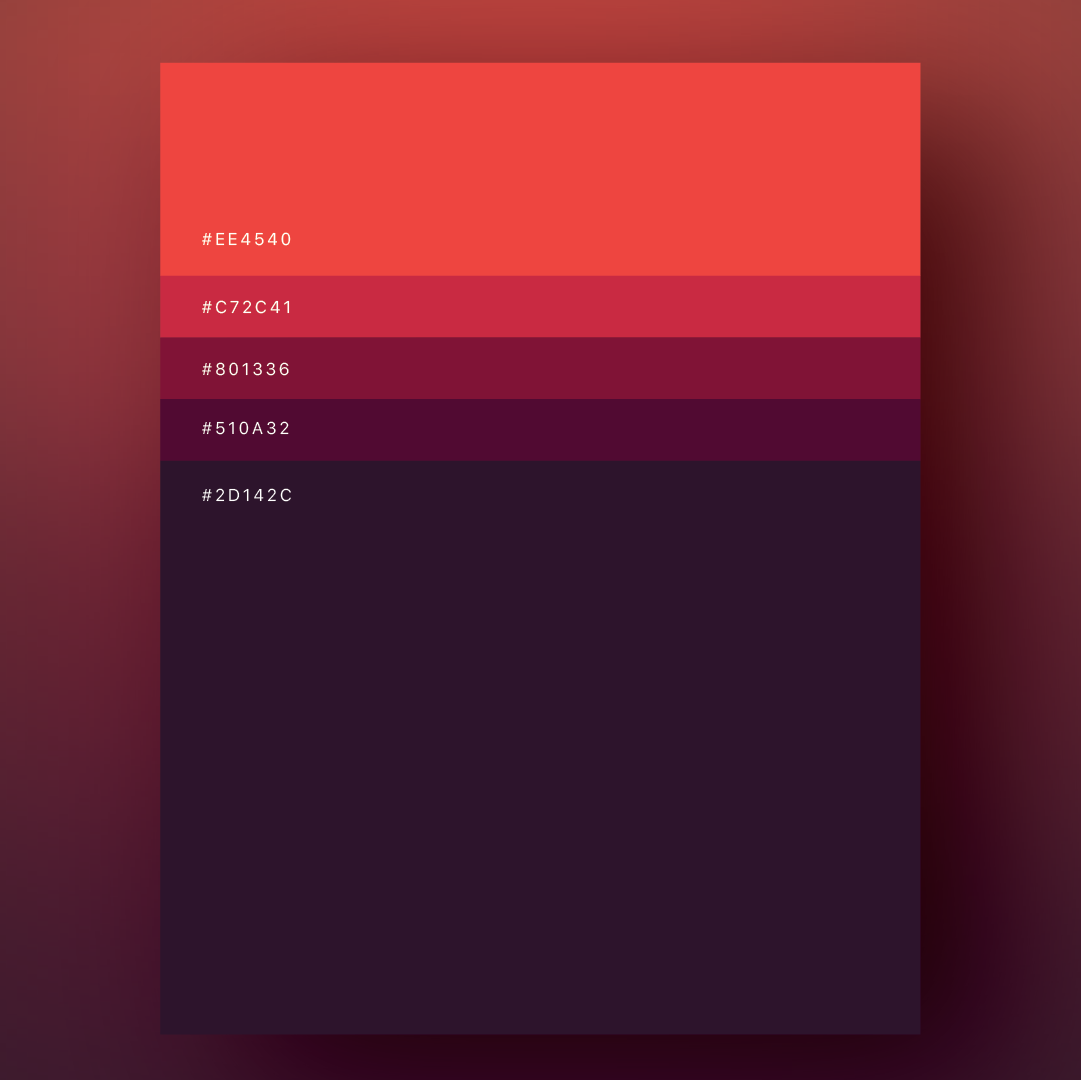
\includegraphics[width=1.0\textwidth]{./images/colorPalette}
    \caption{Color Palette of Trale Messenger}
    \label{fig:colorPalette}
\end{figure}

\subsection{Typography}\label{subsec:typography}
Typography is more than just selecting a good-looking typeface.
Typography is the foundation of how we communicate to other human beings.
It is about contrast, clarity, visual interest drawing the attention of viewers to the important things.
We determined that we should look for a typeface that is great for digital purposes, available in multiple weights, so
we could utilize it in various ways and easily readable.

We decided to go with \textbf{Helvetica Neue} - a sans-serif typeface.
The typeface has been developed in 1957 by Max Miedinger and Eduard Hoffmann and is as of today a widely used font
across print and digital assets as it is perfectly readable.
It is available in various weights and variations as shown in~\ref{fig:figure4}.

\begin{figure}
    \centering
    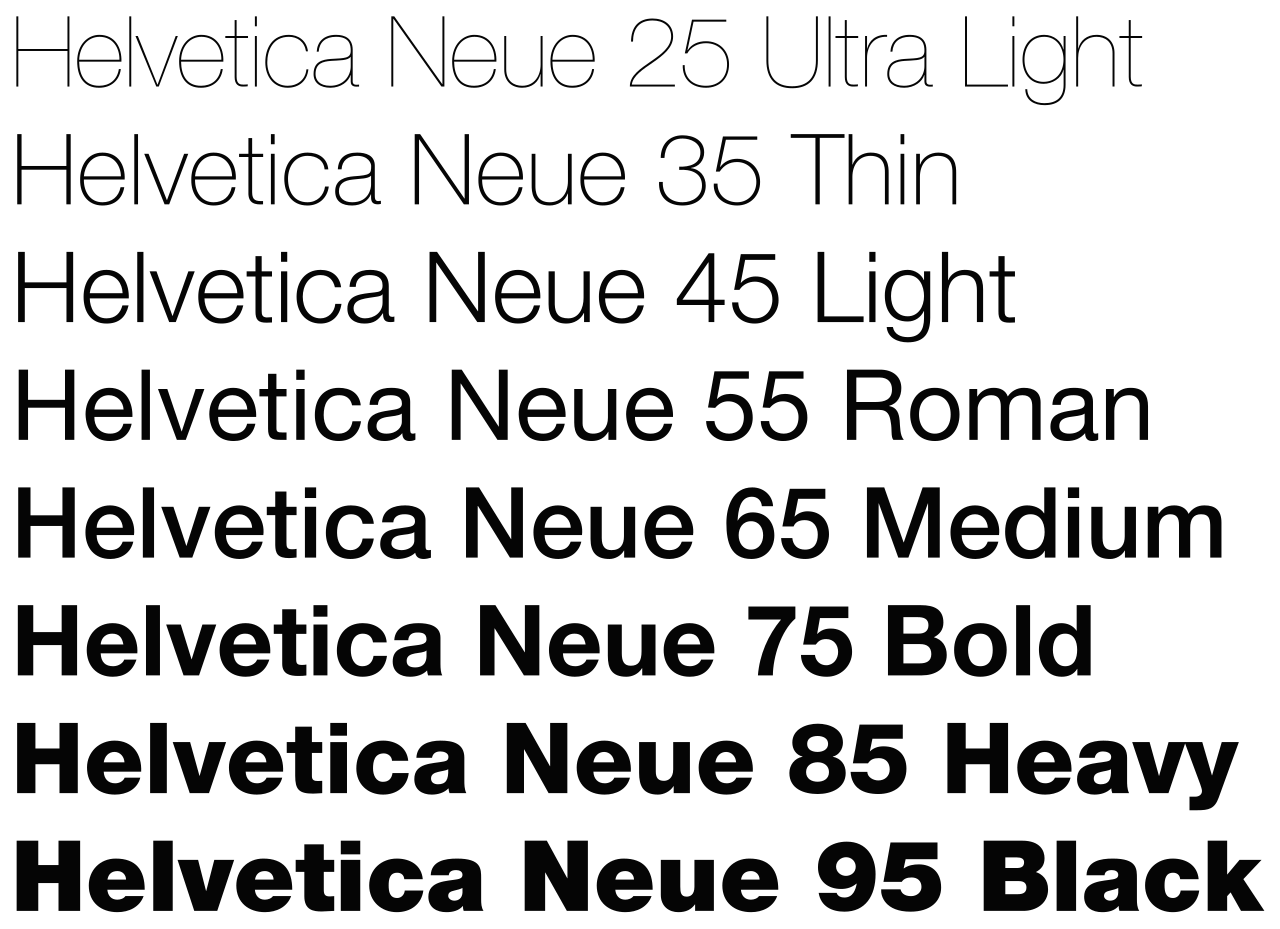
\includegraphics[width=1.0\textwidth]{./images/helvetica-neue}
    \caption{Font: Helvetica Neue}
    \label{fig:figure4}
\end{figure}

Typography is also about spacing of letters, line distance, alignment of text and much more.
In most cases we decided to stick with the default properties and left aligned text as it is the easiest to read.

\section{Wireframes}\label{sec:wireframes}

Based on our preceding analysis we have created several wireframes which match with our guidelines.
Please refer to our \hyperref[ch:wireframes]{\textbf{appendix}} section for a detailed view of our wireframes.
